\documentclass[12pt]{article}

\usepackage{enumerate}
\usepackage{rotating}
\usepackage{multicol}
\usepackage{multirow}
\usepackage{graphicx}
\usepackage{fullpage}
\usepackage{subfigure}
\usepackage{setspace}
\usepackage{listings}
\usepackage{lastpage}
\usepackage{mathtools}
\graphicspath{{./images/}}

% for references
\usepackage[pagebackref=false,colorlinks,linkcolor=blue,citecolor=magenta]{hyperref}
\usepackage[nottoc]{tocbibind}
\usepackage{fancyhdr}
\setlength{\headsep}{25pt}

\pagestyle{fancy}
\fancyhf{}
\lhead{\lr{Digital Image Processing}}
\rhead{آزمون میانترم}
\cfoot{صفحه \thepage\ از \pageref{LastPage}}
\lfoot{نیمسال مهر 00-99}
\rfoot{حمیدرضا ابوئی مهریزی}


% xepersian
\usepackage[extrafootnotefeatures]{xepersian}
\settextfont[Scale=1.2]{B Nazanin}
\setlatintextfont{Times New Roman}

\renewcommand{\labelitemi}{$\bullet$}

\begin{document}
	\doublespacing
	\begin{titlepage}
		\paragraph*{}
		\centering
			
			
			{\small به نام او}\\
			\vspace{1cm}
			\includegraphics[width=0.12\paperwidth]{aut.png}
			\hspace{2.5cm}
			%\includegraphics[width=0.15\paperwidth]{DIP}
			\hspace{2.5cm}
			\includegraphics[width=0.12\paperwidth]{bme}\\
			\vspace{2cm}
			{\Huge پردازش تصویر}\\
			\vspace{2cm}
			{\large استاد : دکتر حامد آذرنوش}\\
			\vspace{0.5cm}
			{\small  دانشجو :‌ حمیدرضا ابوئی}\\
			\vspace{0.5cm}
			{\small شماره دانشجویی : 9733002}\\
			\vspace{0.5cm}
			{\small آزمون میانترم}\\
			\vfill
			{\tiny نیمسال مهر 00-99}
	\end{titlepage}
	\thispagestyle{plain}
	\tableofcontents
	\newpage
	%\onehalfspacing
	\doublespacing
	\section{سوال اول}
		\subsection{توضیحات تکمیلی روند کد}
			ابعاد تصویر برابر است با 
			2912  ,  2912
			و تصویر 
			\lr{retina}
			دارای ۳ کانال است 
			و نوع داده ی پیکسل ها از نوع
			\lr{uint8}
			 می باشد ؛ بنابراین حجم تصویر ما به این صورت خواهد بود :
			 
			 $ 2912 \times 2912 \times 3 \times 8bits = 203,513,856 bits = 25,439,232Bytes \approx 25MBytes  $
			 
			 در نمودار هیستوگرام ، داده های مساله (شدت های پیکسل های تصویر ) به صورت کلی و دسته بندی شده به نمایش در می‌آید. محور افقی نشان دهنده‌ی میزان شدت پیکسل ها از صفر تا ۲۵۵ و محور عمودی نشان دهند‌ه‌ی فراوانی ( و یا تعداد پیکسل ها ) شدت هاست .
			 هیستوگرام به خوبی می‌تواند میزان پراکندگی شدت های تصویر را نشان دهد و همچنین میتواند اطلاعات زیادی از قبیل میزان روشنایی حقیقی تصویر ( فارغ از نوع نمایشگر ) ، میزان نوردهی تصویر ، تشخیص 
			\lr{ over exposure , under exposure}
			تشخیص میزان حدودی کنتراست و...
			
			برای یافتن قسمت شبیه تصویر بزرگ تر به کوچک تر، تصویر بزرگتر را می گردیم و به پنحره های کوجک اندازه ی تصویر کوچک تقسیم میکنیم و این پنجره را با گام هایی ( ۸۰ تا ) در طر تصویر بزرگ می لغزانیم و هیستوگرام آن را محاسبه می‌نماییم. و مقایسه میکنیم. و جایی که بیشترین شباهت را دارد مشخص می نماییم . حال برای دقت بیشتر از ۸۰ ، میتوانیم این عملیات را با دقت بیشتر حول مختصاتی که به دست آوردیم با طول گام کوتاه تر انجام دهیم تا مقدار دقیق تری را به ما بدهد.
		
			در قسمت آخر نیز در تابع تعریف شده ابتدا تصویر ۸ بیتی را به صورت باینری تبدیل کرده و سپس بیت های مختلف آن را به عنوان صفحه های مختلف برداشت میکنیم  
			همانطور که مشخص است، کلیات تصویر، بیشتر در بیت های با ارزش بیشتر مشخص است و هرچه به بیت های کم ارزش تر می‌رسیم فرکانس تغییرات بیشتر شده و تصویر نشان داده شده کمتر به تصویر اصلی شبیه است .
		\subsection{ورودی برنامه}
		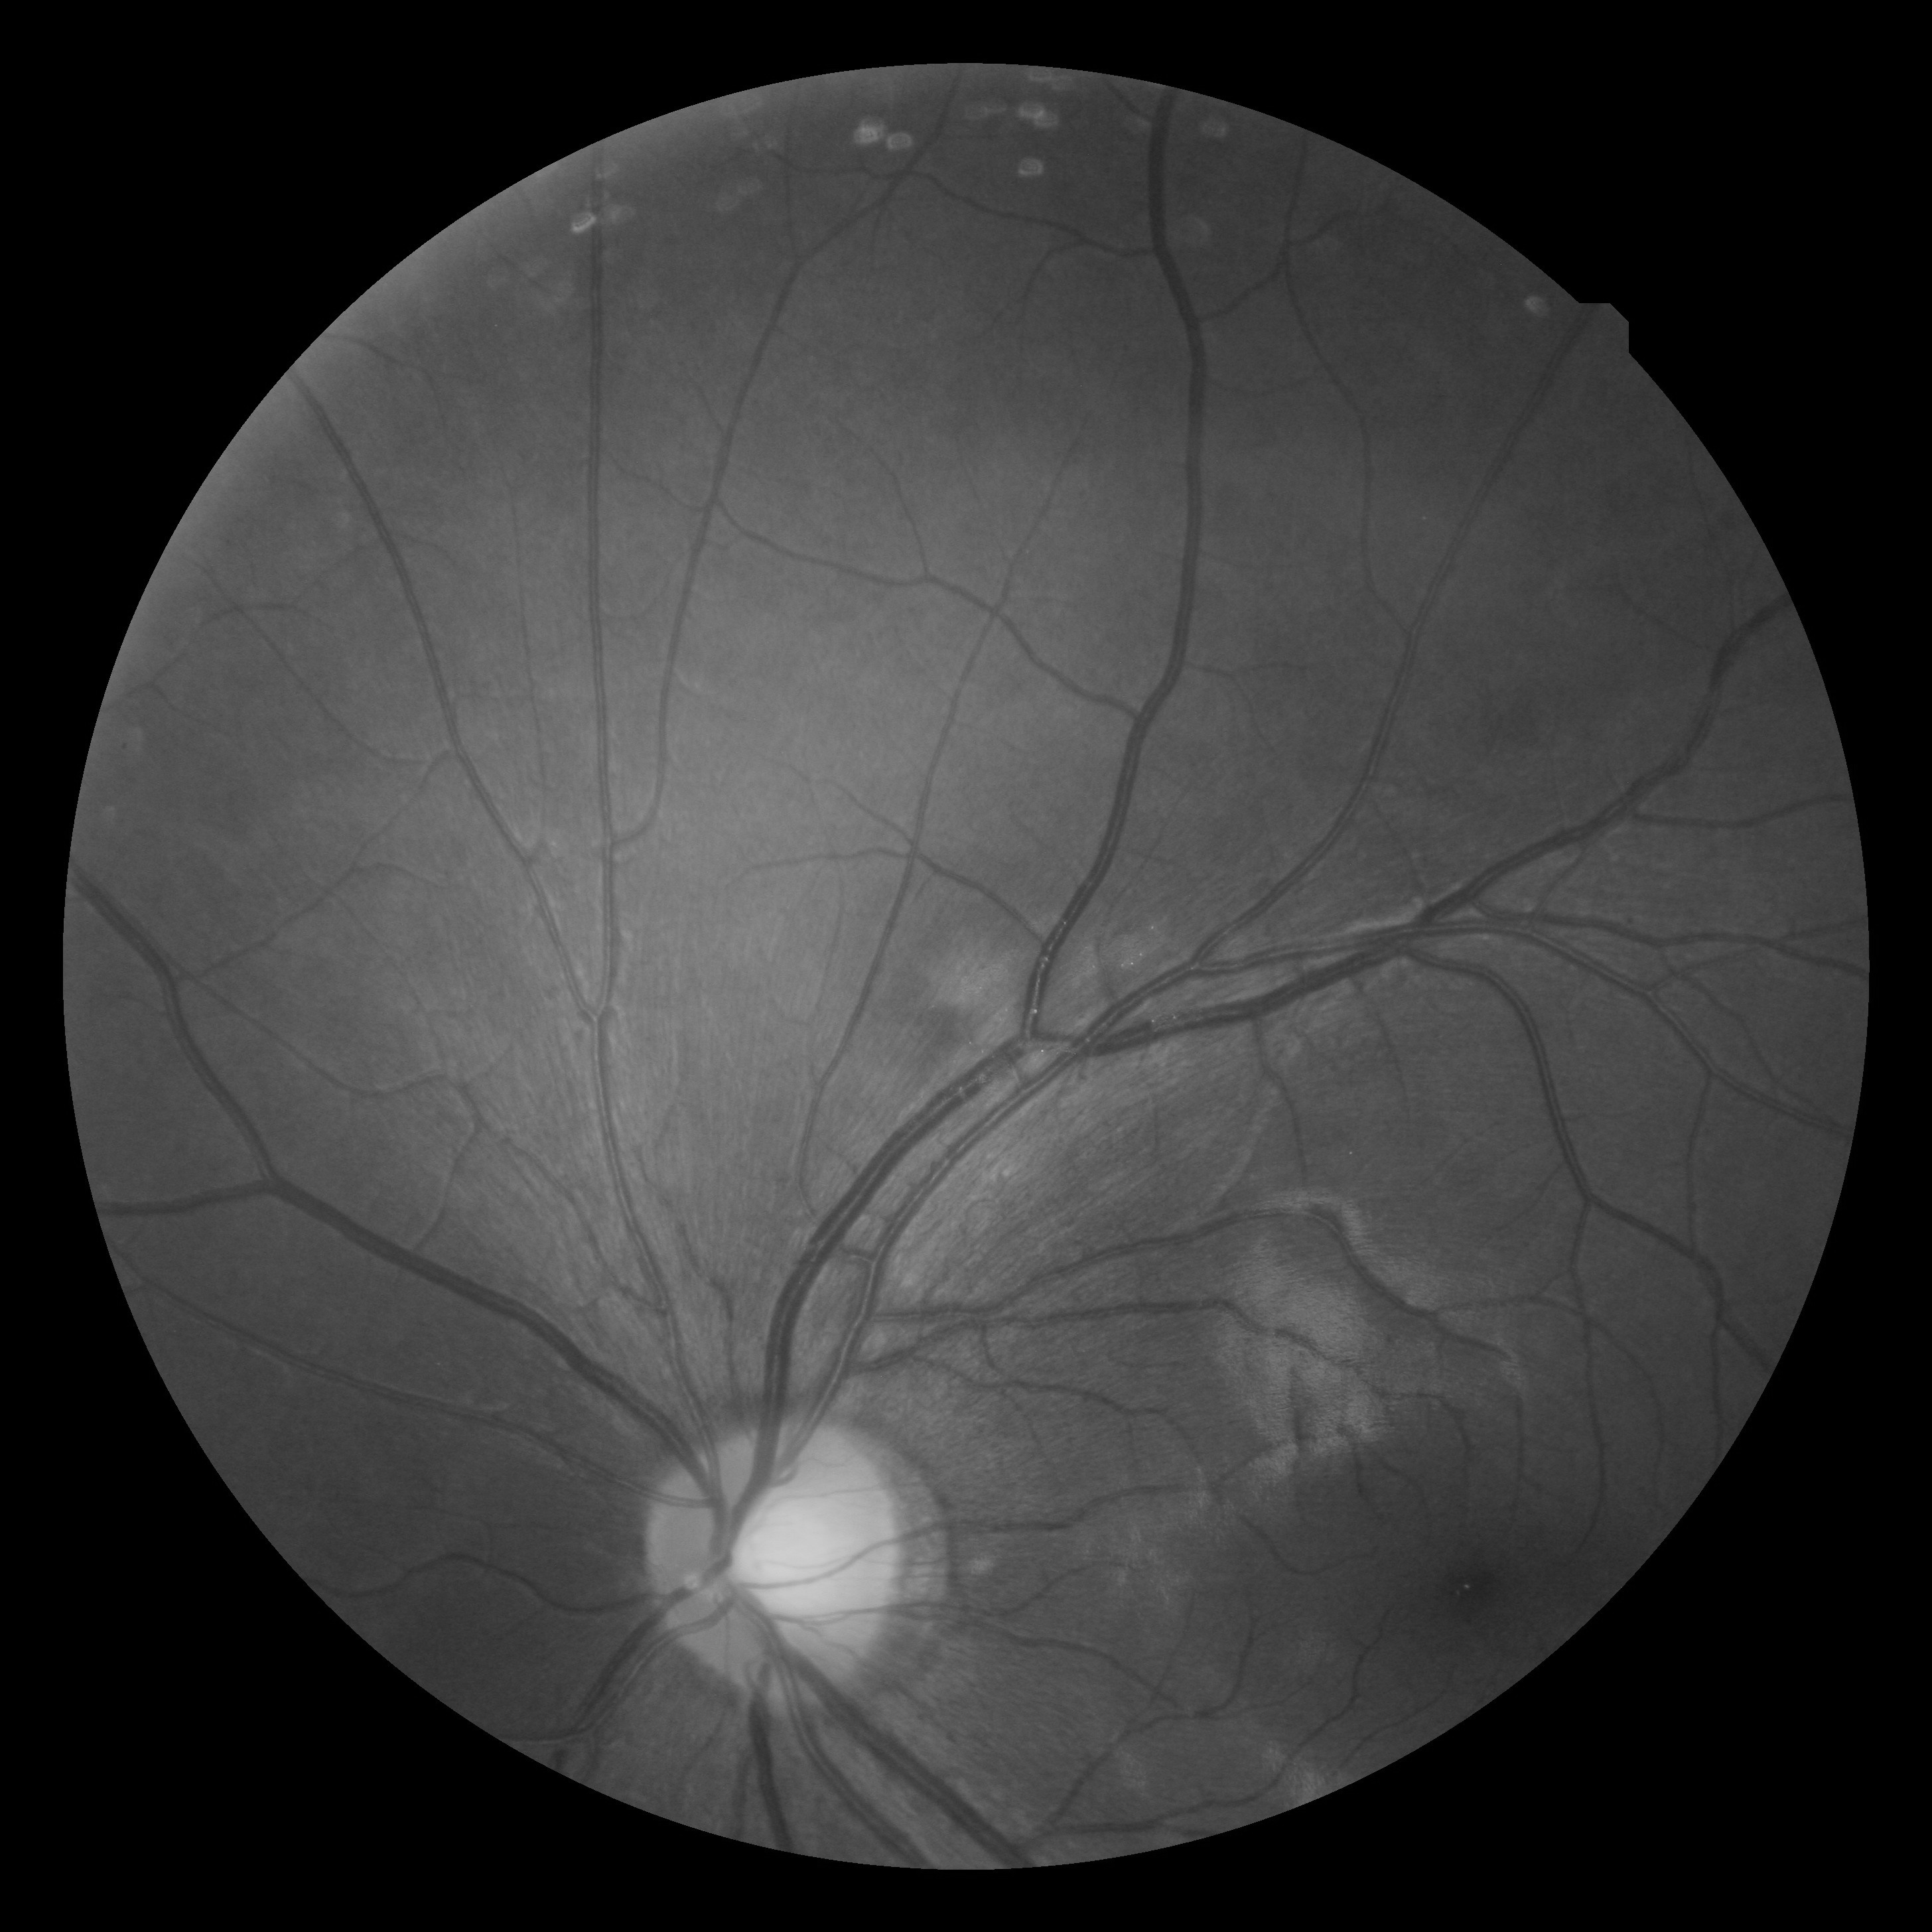
\includegraphics[width=10cm]{inputs/retina.jpg}
		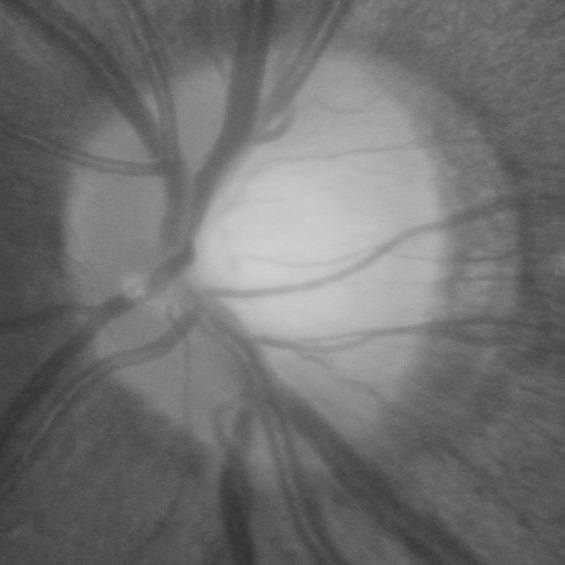
\includegraphics[width=5cm]{inputs/retina_sub.jpg}
		\subsection{خروجی برنامه}
		\lr{shape  2912  ,  2912\\
			channel :  3\\
			<class 'numpy.uint8'>\\}
		
		\includegraphics[width=17cm]{1-0}
		
		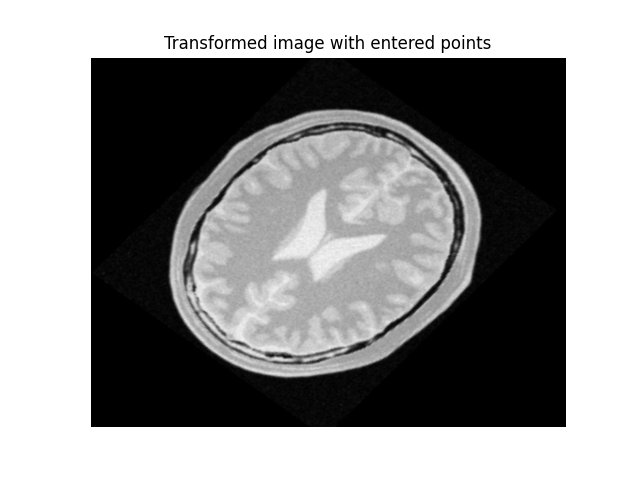
\includegraphics[width = 13 cm]{1-1}\\
		\includegraphics[width = 17 cm]{1-2}
		
		
		\newpage
		
		\section{سوال دوم }
		\subsection{توضیحات تکمیلی روند کد}
	دوره ی تناوب تابع سینوس برابر است با 
	$2 \times \pi $
	.
	حال ما میخواهیم تابع‌مان بدین صورت عمل کند که در بازه ی 
	$ [ 0 , (L-1) ] $
	همواره صعودی باشد . میدانیم که مقدار سینوس در صفر برابر صفر است و باید 
	$a$
	را چنان بیابیم که حداکثر مقدار سینوس در انتهای بازه برابر با ۱ شود . یعنی داخل سینوس به 
	$\frac{ \pi}{2} $
	برسد .

بدین منظور 
$a$
را بدین صورت به دست می‌آوریم :
			$a\times (L-1) = \frac{\pi}{2} $
			
			$a=\frac{\pi}{2 \times (L-1)}$
			
			$s(r) = (L-1)sin(\frac{\pi}{2 \times (L-1)} \times r)$
	
	این تابع تبدیل برای تصاویر تاریک مناسب‌تر است. همانطور که در منحنی تبدیل مشخص است ، کنتراست شدت های کم تصویر تحت این تبدیل ، بیشتر می‌شود و همچنین کنتراست تصویر در شدت های بالا کاهش می‌یابد . در کل نیز میزان شدت پیکسل های تصویر بیشتر است زیرا در نمودار منحنی تبدیل کل نمودار بالاتر از نیمساز است . بنابراین در تصوبر 
	\lr{CT\_2}
	شدت پیکسل ها که افزایش می‌یابد ،کنتراست تصویر کاهش می یابد و در نتیجه تصویر بدتر می‌شود. 
	همچنین از روی هیستوگرام تصویر نیز میتوان به این موضوع پی برد :
	\includegraphics[width=17cm]{2-1.png}

	
	
		\subsection{ورودی برنامه}
		\includegraphics[width=5cm]{inputs/CT_1.png}
		\includegraphics[width=5cm]{inputs/CT_2.png}
		\subsection{خروجی برنامه}
		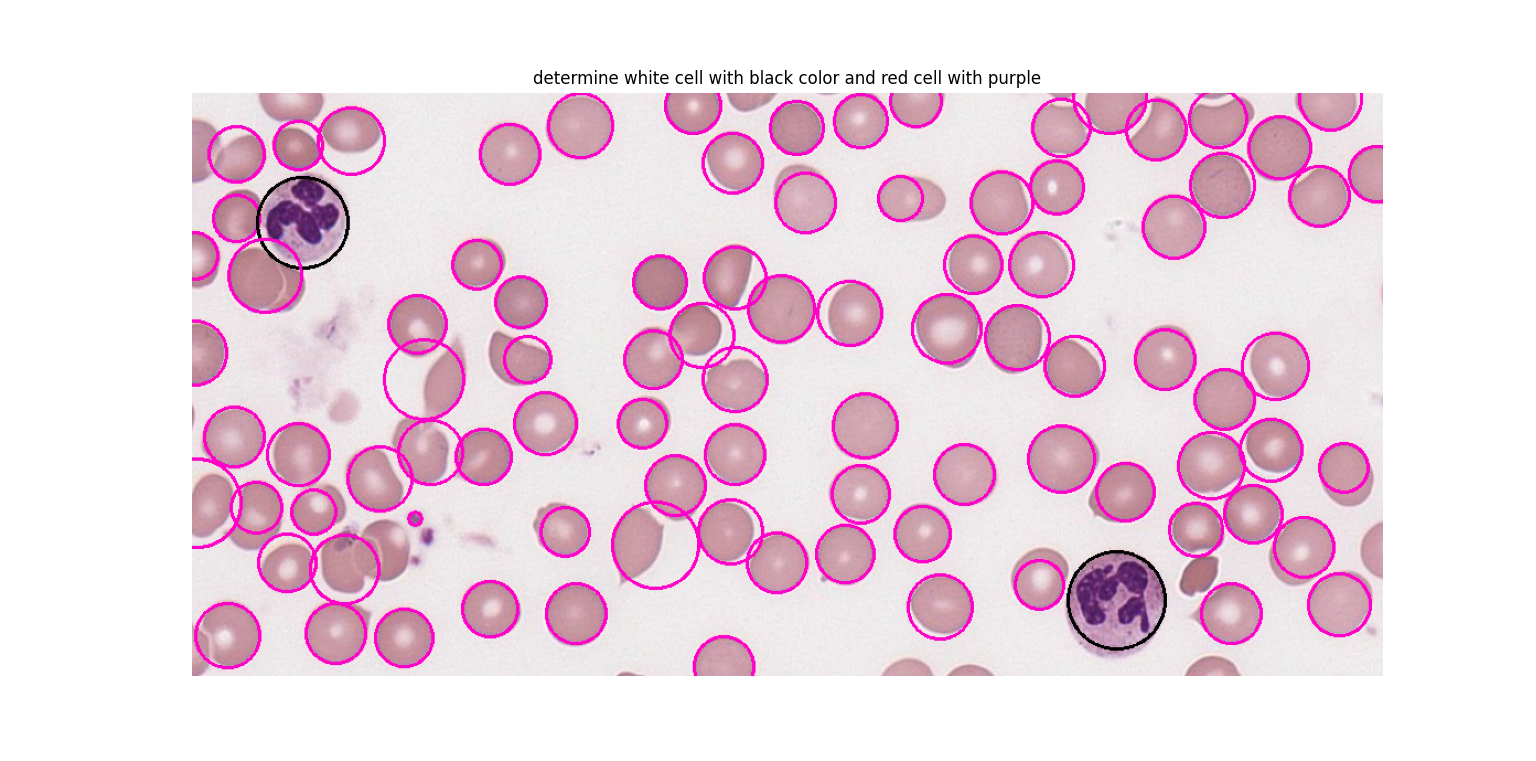
\includegraphics[width=8cm]{2-2.png}
		\includegraphics[width=8cm]{2-3.png}
		
		\newpage
		
		\section{سوال سوم }
		\subsection{توضیحات تکمیلی روند کد}
	تصحیح فایل داده شده
	اولا برای خواندن تصویر به صورت خاکستری باید یک 0 در خط
	
	\lr{img = cv2.imread('lung.png',0)}
		
		گذاشته شود
		ثانیا فیلتر 
		\lr{blur}
		یک فیلتر خطی است که برای حذف نویز فلفل نمکی مناسب نیست زیرا صرفا آن را گسترده می‌کند 
		به جای آن میتوانیم از فیلتر غیر خطی و آماری 
		\lr{median}
		\lr{(cv2.medianblur)}
		استفاده کنیم .
		
		
		نکته ی دیگر آن که در فیلتر سوبل برای گرادیان گیری برای این که پاسخ بهتری بدون محاسبات اضافه تر بگیریم نیاز است که 
		\lr{ddepth }
		را در ۸ بیت (یعنی 
		\lr{v2.CV\_8U}
		) به دست محاسبه نماییم 
		و نکته ی دیگر آنکه بهتر است در هنگام نمایش دادن تصویر در 
		\lr{matplotlib.pyplot.imshow}
		مشخصات 
		\lr{vmin , vmax}
		را 255 و 0 در نظر بگیریم .
		
		نکته ی قابل ذکر راجع به بالا روند یا پایین رونده بودن وجود دارد آن است که وقتی ما فیلتر سوبل 
		
		$
		\begin{bmatrix}
			1 & 2 & 1 \\
			0 & 0 & 0 \\
			-1 & -2 & -1 \\
		\end{bmatrix}
	$

را اعمال می نماییم ، به ما یک تصویر با مقادیر مثبت و منفی می‌دهد . حال برای نمایش این سه راه وجود دارد. 
\begin{itemize}
	\item
 مقادیر منفی را حذف نماییم
	\item 
	مقادیر منفی را قرینه کنیم یا از روش 
	$G = \sqrt {G^2 }$
	استفاده نماییم که هر دو لبه ی بالا رونده و پایین رونده را می‌دهد 
	\item 
	کوچکترین مقدار را برابر با 0 و بزرگترین عدد را برابر ۲۵۵ قرار دهیم . که رنگ پایه تصویر ما خاکستری می شود.
\end{itemize}

به نظر می‌رسد که منظور تدریس یار از این سوال صرفا همان گزینه ی دوم میباشد که هم لبه های بالارونده و هم پایین رونده را شامل می‌شود. 
 
 
 اصلاحیه :‌
 
 به دلیل کم بودن زمان، برخی نکات در این قسمت ذکر می شود:
  در مستندات 
  \lr{open cv}
   و کتاب های نوشته شده مانند 
  \lr{Learning OpenCV by Bradski and Kaehler}
  آمده است که برای از دست نرفتن اطلاعات لازم است حتما برای 
  \lr{ddepth}
  حداقل از متغیر هایی با تایپ 32 بیتی علامت دار استفاده شود. 
 بنابراین در کد ارسال شده برای اطمینان بیشتر از عمق 
 \lr{float64}
 استفاده شده است. در چیزی که در بالا آمده است یعنی 
 \lr{ddepth = cv.CV\_8U}
 مقداری از اطلاعات مساله از دست می رود و برای مثال همان قسمت پایین رونده از داده ها حذف می شود بنابراین کد به همان 
 \lr{float64}
 تبدیل شده است . بدین ترتیب نیاز است که برای یافتن خروجی دلخواه، ابتدا مقادیر منفی به دست آمده را مثبت کرده با قدر مطلق گیری و سپس متغبر ها را به 0 تا 255 اسکیل کرده و سپس داده را به آنچه مساله خواسته یعنی 
 \lr{uint8}
 تبدیل نماییم.  
 
 
		برای این که گرادیان را  از هر دو جهت عمودی و افقی بگیریم یک راه آن است که جداگانه از تصویرمان در جهت افقی و در جهت عمودی گرادیان گیری کنیم و سپس آن ها را با هم جمع کنیم , 
		البته قدر مطلق گرفتن از هر کدام از گرادیان ها و سپس جمع کردن و یا توان دو رساندن و سپس رادیکال گرفتن از جمع آنها  نیز میتواند راهگشا باشد .
		یک راه دیگر نیز در مستندات آمده است که با جمع کردن وزنی این دو میتوان نتیجه گرفت که به طور معمول عدد 5.0 در نظر گرفته می‌شود و میتوان آن را تغییر نیز داد.
		تصویر زیر نمایش دهنده ی آن است:\\
		\includegraphics[width=10cm]{3-both.png}
		
		\subsection{ورودی برنامه}
		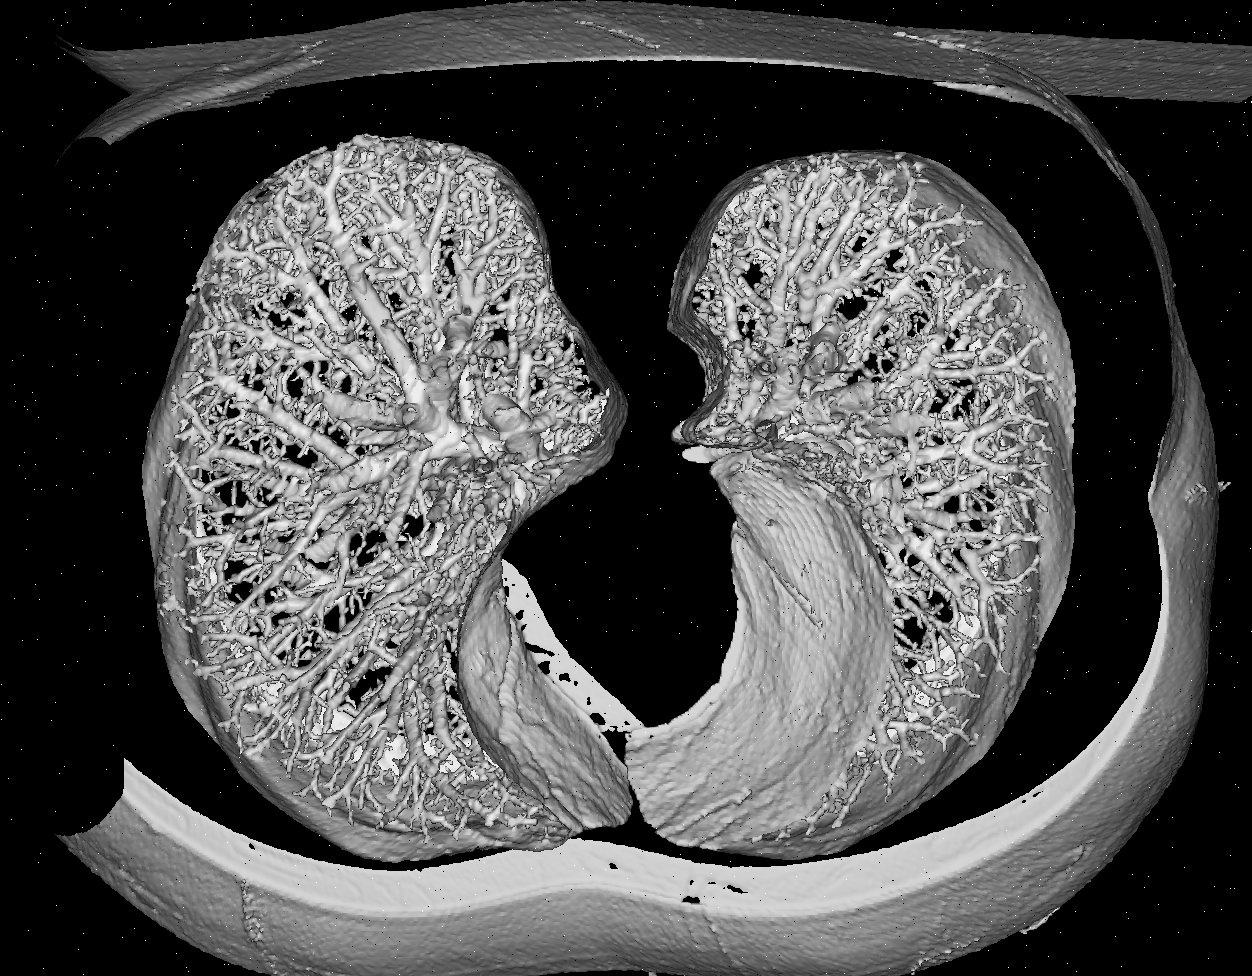
\includegraphics[width=5cm]{inputs/lung.png}
		\subsection{خروجی برنامه}
		\includegraphics[width=17cm]{3-1.png}
		
		
		\newpage
		
		\section{سوال چهارم }
		\subsection{توضیحات تکمیلی روند کد}
	برای یافتن نقاطی که نویز را به سیستم ما وارد می‌کند راه های مختلفی وجود دارد.
	یکی از این راه ها که در کد ارسالی از آن استفاده شده است یافتن این نقاط بر حسب این که شدت این نقاط در تبدیل فوریه ی ما بیشتر از سایر نقاط اطرافش به جز در اطراف مرکز تصویر است .
	بنابراین مطابق شکل زیر چهار بار ماکزیمم مقدار تصویر و نقاط آن را محاسبه میکنیم که همان نقاطی را به ما میدهد که نویز روی تصویر ما انداخته است.
	
	\vspace{1cm} 
	
	\includegraphics[width=5cm]{4-1.png}
		\subsection{ورودی برنامه}
		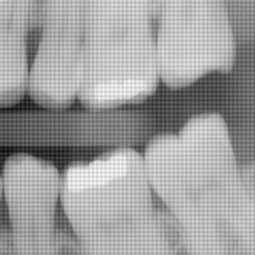
\includegraphics[width=7cm]{inputs/xray_checkered.png}
		\subsection{خروجی برنامه}
		\includegraphics[width=17cm]{4.png}\\
		
		با تشکر
		\newpage


\end{document}
